\documentclass[12pt]{article}

\usepackage[hungarian]{babel}
\usepackage{t1enc}
\usepackage[utf8]{inputenc}
\usepackage[margin=2.5cm]{geometry}
\usepackage{setspace}
\usepackage{graphicx}
\usepackage{float}
\usepackage{hanging}
\PassOptionsToPackage{hyphens}{url}\usepackage{hyperref}
\usepackage{amsmath}

\hypersetup{
    colorlinks,
    citecolor=black,
    filecolor=black,
    linkcolor=black,
    urlcolor=blue
}

\graphicspath{ {./figs/} }
\setlength{\belowcaptionskip}{5pt plus 3pt minus 2pt}

\setstretch{1.5}

\begin{document}

\begin{titlepage}
	\begin{center}
		\vspace*{5cm}
		
		\Huge
		\textbf{Kockázatmodellezés és -előrejelzés}
		
		\vspace{2cm}
		
		\LARGE
		Salamon András, Szilágyi Gergő
		
		\vfill
		
		\Large
		Hitelek és kockázatok makro és mikro szinten \\

        \vspace{1cm}
        
        2023. tavaszi félév
            
    \end{center}
\end{titlepage}

\newgeometry{margin=2.5cm}

\tableofcontents

\clearpage

\listoffigures

\clearpage

\section*{Git URL}

A git repository, ahol dolgoztunk, \href{https://github.com/MaboSzate/beadando_SA_SzG}{ezen a linken} érhető el.

\section{Historikus VaR}

A Value at Risk (VaR) egy mutató, amivel egy eszköz, vagy egy portfólió lehetséges veszteségét lehet számszerűsíteni. Azt mutatja meg, hogy adott konfidenciaintervallum mellett legrosszabb esetben mennyit veszítünk a befektetésünkkel. A VaR számtásának egyik módja a historikus VaR, amikor múltbeli adatokból indulunk ki. A feladatunk ennek kiszámtása volt egy kételemű portfólióra. Két ETF-et, a MOO-t és a VOO-t választottuk ehhez.

A két eszköznek összesen 100 féle súlyozását néztük meg, ami az egész $[0,1]$ intervallumot lefedte. Így megkaptuk azt az optimális súlyozást, ami a legjobb historikus VaR értéket adja.

\begin{figure}[H]
	\centering
	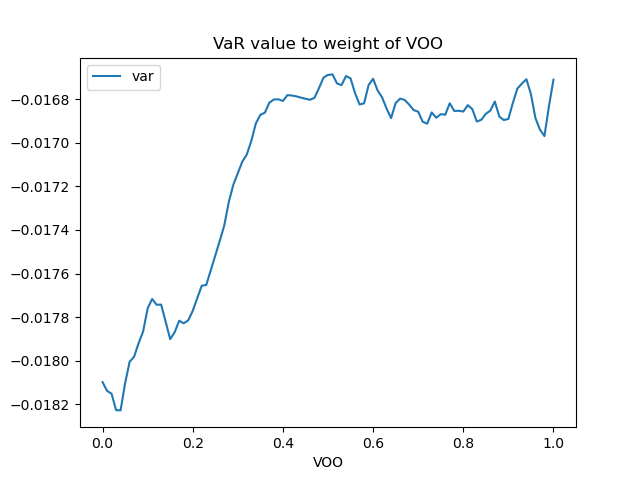
\includegraphics[scale=0.9]{var}
	\caption{VaR értéke a VOO súlyának függvényében, 95\%-os konfidenciaszint mellett}
\end{figure}

Ahogy az ábrán az látható, kb. 0,2\%-os VaR eltérést tudunk elérni az eszközök optimális súlyozásával. A legmagasabb VaR érték -1,67\%, ez azt jelenti, hogy a hozamok 95\%-a ennél magasabb volt. Ehhez majdnem fele-fele arányban kell venni a két eszközt: a VOO súlya 0,51, a MOO-é 0,49.



\section{Szimulált VaR}

Az előző VaR-ral ellentétben ebben a feladatban nem a historikusan meghatározott kvantilis értékét számoltuk ki, hanem a portfólió várható hozamát és volatilitását határoztuk meg, és ezen értékek alapján határoztuk meg az ezen paramétereknek megfelelő normális eloszlás megfelelő kvantilisát. Ezt az értéket tekintettük VaR-nak.

Ahogy az előző feladatban, itt is 95\%-os konfidenciaszintet használtunk, azonban most a VaR értékét és két ETF közötti korreláció kapcsolatát vizsgáltuk. Ehhez a múltbeli adatok alapján meghatároztuk a két ETF várható hozamát és volatilitását, amelyből egy feltételezett korreláció mellett meghatároztuk a portfólió várható értékét és volatilitását. A portfólióban az ETF-ek a volatilitásuk reciprokával arányos súlyt kaptak. Így az adott súlyvektor mellett a portfólió várható hozama a súlyvektor és az eszközök hozamának a skalárszorzata, volatilitása pedig a kovarianciamátrixból és a súlyvektorból kiszámított kvadratikus alak gyöke.

A fenti számításokat különböző korrelációk mellett elvégezve az alábbi ábrán látható értékeket kaptuk. Ahogy az azonnal szembeötlik, minél erősebb a negatív korreláció, annál nagyobb a VaR értéke, így az az érték, amit a portfóliónk legfeljebb 5\%-kal elveszíthet, abban az esetben lesz a legalacsonyabb, ha a két ETF közötti korreláció -1. Az ábrán az is látható, hogy ebben az esetben a VaR már pozitív értéket vesz fel, azaz a portfólió nem veszíthet az értékéből, ha hihetünk a számításainknak.

Az eredmény abból a szempontból nem meglepő, hogy minél inkább negatívan korrelál a két eszköz, annál inkább ki tudják egymást ellensúlyozni: ha az egyik ETF értéke bezuhanna, akkor a másiké megnő, így kompenzálva azt a veszteséget, amit elszenvednénk. Minél inkább pozitívan korrelálnak, annál nagyobbat veszíthetünk, mivel ebben az esetben együtt zuhannak az ETF árfolyamai.

\begin{figure}[H]
	\centering
	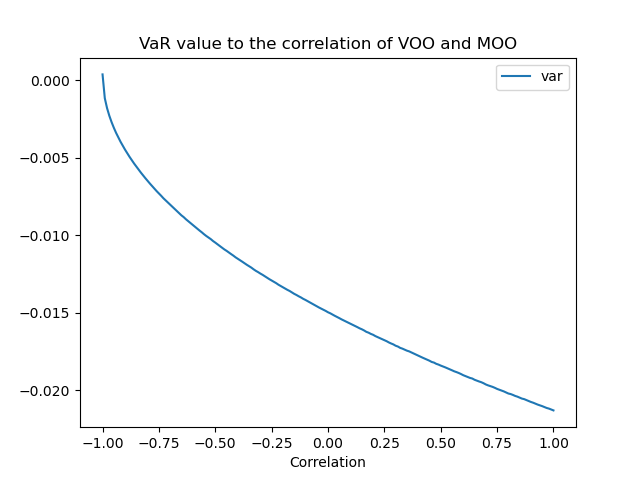
\includegraphics[scale=0.9]{sim_var}
	\caption{VaR értéke a VOO és MOO közötti korreláció függvényében.}
\end{figure}


\section{EWMA}

Az EWMA (Exponentially Weighted Moving Average) segítségével szimulálható a pénzpiacokon megfigyelhető volatilitásklasztereződés. Eszerint azokat a napokat volatilisebb napok követik, amelyeken jobban ingadozik az árfolyam, valamint ez fordítva is igaz, a nyugodtabb napokat nyugodtabb napok követik. Az EWMA-ban a késleltetett loghozamok négyzetét exponenciálisan csökkenő súlyokkal súlyozzuk, amelyek összegét egyre normáljuk. A késleltetés minden esetben 100 volt. Az alábbi ábrán látható az összefüggés a decay faktor értéke és a késleltetett hozamnégyzetek között. 

\begin{figure}[H]
	\centering
	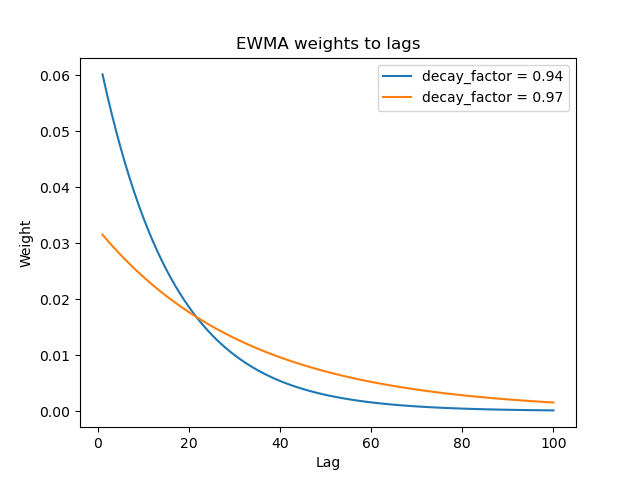
\includegraphics[scale=0.9]{ewma_weights}
	\caption{EWMA súlyok különböző decay faktorok mellett}
\end{figure}

Azt, hogy mennyire gyors az exponenciális csökkenés, a decay faktor értéke határozza meg. Nagyobb decay faktor mellett lassabb a csökkenés, és mivel egyre normáljuk a súlyokat, ezért a néhány késleltetéses tagok kisebb súlyt kapnak, mint nagyobb decay faktor mellett. Alacsonyabb decay faktor mellett drasztikusabb a csökkenés gyorsasága, és ekkor a korai késleltetések súlyai nagyobbak, mivel a gyors csökkenés miatt, amikor egyre normáljuk az összeget, nem visznek el akkora súlyt a későbbi késleltetések. 

Az alábbi ábrán látható a MOO ETF-re számolt volatilitások a kétféle decay faktor mellett.

\begin{figure}[H]
	\centering
	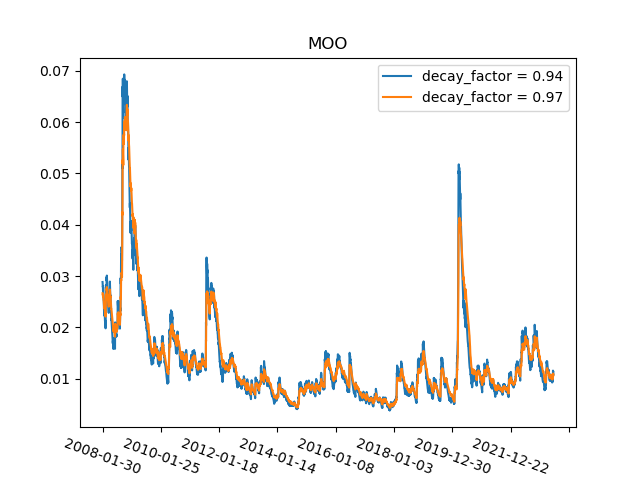
\includegraphics[scale=0.9]{ewma_moo}
	\caption{EWMA a MOO idősoros adatokon a két decay faktor mellett}
\end{figure}

Ahogy az ábrán látható, nagyobb decay faktor mellett kisebb az előrejelzett volatilitás. Azonban ebben az esetben a volatilitások jobban klasztereződnek, mivel nem olyan nagyok a kilengések, így közelebb maradnak egymáshoz az egymást követő napok volatilitásai.


\section{Machine Learning}

Végezetül készítettünk egy lineáris regressziós modellt is a jövőbeli variancia múltbeli adatokból történő előrejelzésére. A célváltozó a napi loghozam négyzete, a magyarázó változók pedig a loghozamok négyzete laggolva (eltolva), az EWMA módszeréhez hasonlóan. Kezdetben 10 lagot csináltunk, hogy a számítógépeink le tudják futtatni az optimalizációt.

Az optimális fokszám megtalálásához hiperparaméter-keresést végeztünk, ennek az eredménye az lett, hogy a legalacsonyabb MSE az elsőfokú modell mellett volt. A fokszám növekedésével jelentősen emelkedett az MSE is, gyorsan egyértelművé vált számunkra, hogy elég csak az elsőfokú polinomos esetet vizsgálnunk. A cross-validation is megerősítette ezt.

A modell egyszerűsödése elsőfokúra lehetővé tette számunkra, hogy hosszabb időtávon vizsgáljuk az adatokat, és, hogy 10 helyett 20 eltolt loghozamvektort használjunk. Így talán jobban használható modellt kaptunk. Az egész adathalmazra alkalmazott modell koefficiensei a következők lettek:
\begin{align*}
        &(0.1301,\; 0.4455,\; 0.106,\; -0.0975,\; -0.0006,\; 0.0760,\; 0.0082,\; 0.1015,\;
        -0.0262,\; -0.0182,\; \\& -0.0183,\; 0.0087,\; 0.0069,\; 0.0149,\; 0.0625,\; -0.0709,\; 0.0341,\; 0.0045,\; -0.0427,\; 0.0107).
\end{align*}
Látható, hogy a legnagyobb koefficiens a második változóhoz, azaz a 2-vel eltolt loghozam-négyzetekhez tartozik. Ez az eredmény azt mondja a számunkra, hogy az előző két nap eseményei vannak a legnagyobb hatással az ETF árának alakulására. Ha csak az előző napot vesszük hozzá, vagy pedig ha több napot is hozzáveszünk, a magyarázóerő kisebb lesz.

A cross-validation alapján ez az eredmény konzisztens a train-test halmazok megválasztásától függetlenül:

\begin{figure}[H]
    \centering
    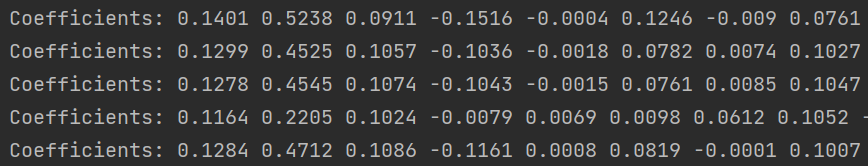
\includegraphics{cross_validation.png}
    \caption{Első 8 koefficiens értéke elsőfokú modellben, 5 különböző train-test set mellett}
\end{figure}

\end{document}














